\chapter{Aufbau}
\label{ch:Funktionsweise und Aufbau}
Die Funktionsweise des Gestikulasers besteht aus der Detektion und Weiterverarbeitung von Lichtsignalen, welche mit einer Geste erzeugt werden. Dabei wird infrarotes Licht von einer LED Quelle durch die Hand reflektiert und mit Hilfe von verschiedenen Photodioden detektiert. Die durch die Photodioden erhaltenen Daten werden dann in einer Software weiterverarbeitet, welche mit Hilfe von Machine Learning die tatsächliche Handgeste erkennt. Von dort aus kann dann jedes beliebige Endgerät angesteuert werden.

\begin{figure}[h]
	\centering
	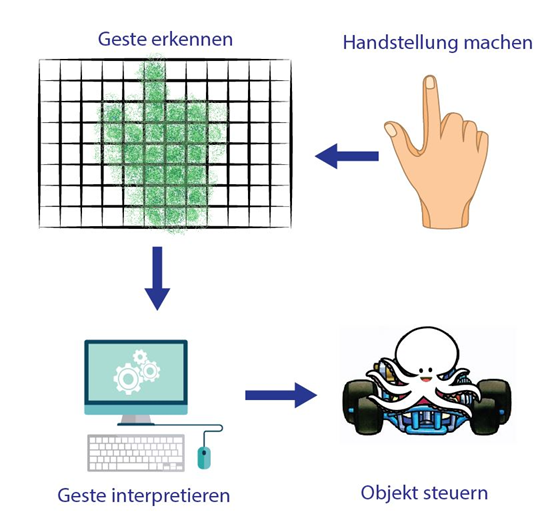
\includegraphics[scale=0.8]{../figures/AblaufGestikulaser.png}
	\caption{\textcolor{red}{Erklärung!}}
	\label{fig:AblaufGestikulaser}
\end{figure}

Der Gestikulaser selbst besteht aus einer Platte, der Photoplatte, welche aus verschiedenen Steckmodulen zusammen gesteckt werden kann. Die Steckmodule bestehen aus einzelnen kleinen Boxen, in welche die Elektronik integriert ist. In der Mitte befindet sich der Oktokommander, welcher durch weitere Detektormodule erweitert werden kann. Auf jedes der Module befinden sich vier Photodioden um das reflektierte Licht zu messen. 

\begin{figure}[h]
	\centering
	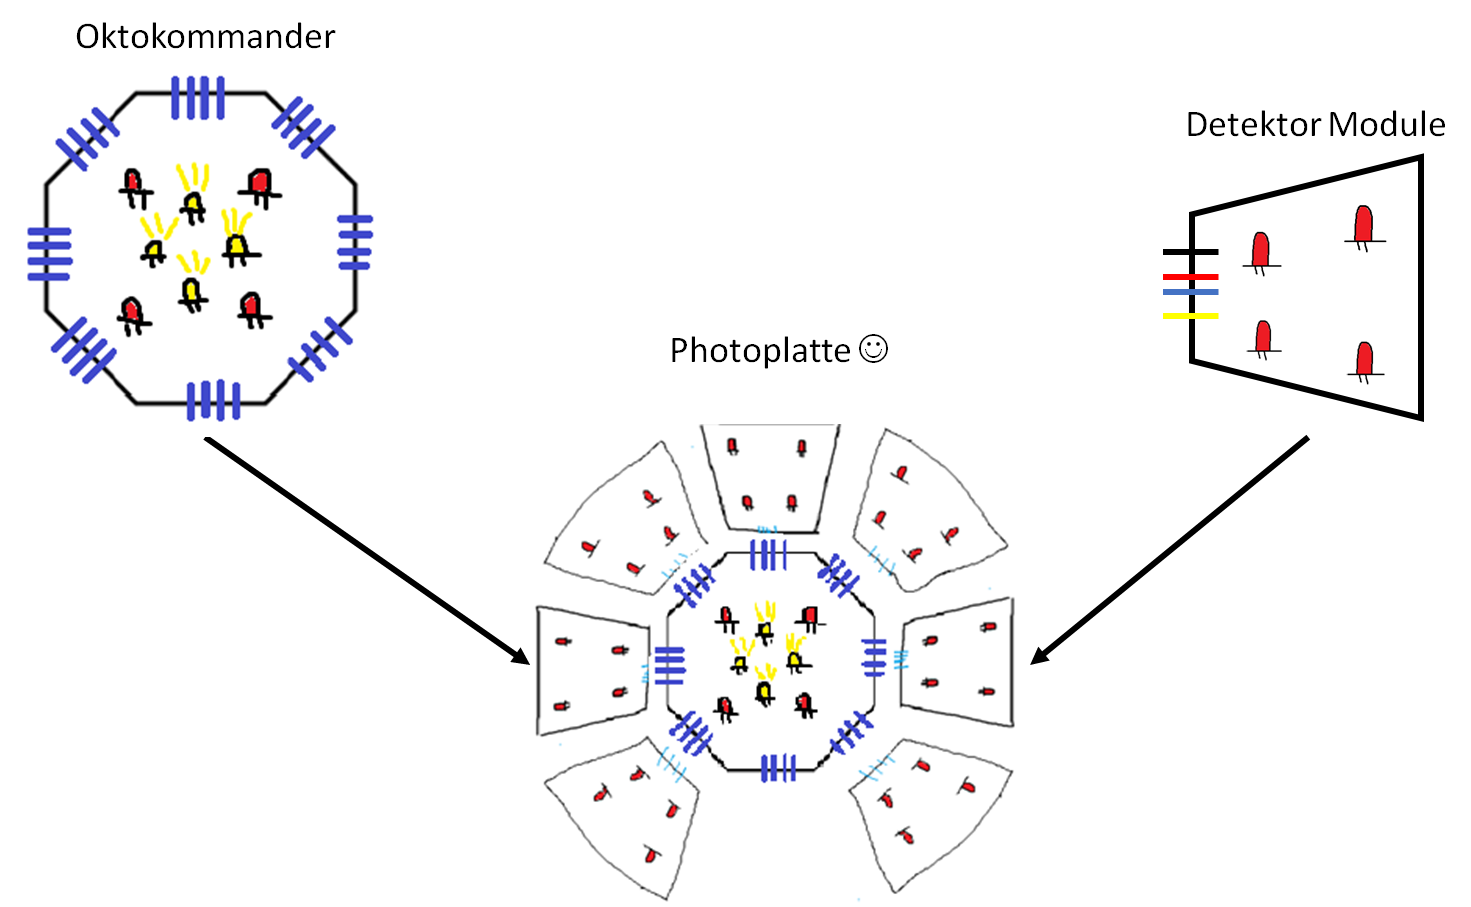
\includegraphics[scale=0.5]{../figures/Photoplatte.png}
	\caption{\textcolor{red}{Erklärung!}}
	\label{fig:Fotoplatte}
\end{figure}

% -------------------------------------------------------------------------------------- %

\section{Oktokommander}
\label{sec:Oktokommander}

Der Oktokommander ist das Steuersystem der gesamten Photoplatte. In ihr befinden sich ein Arduino Micro, welcher die Signale aller Photodioden bearbeitet sowie einen i2c Expander. Durch den i2c Expander ist es möglich, jedes der Photodioden eine eigene Adresse zu zu weisen. Dies ist nötig, um die voneinander unabhängigen Signale der Photodioden richtig zuordnen zu können. Zusätzlich dazu befinden sich auf dem Oktokommander vier Infrarot LEDs sowie vier infrarot Photodioden. Um die vier infrarot Photodioden an zu steuern wird zusätzlich zum i2c Expander noch ein i2c Multiplexer sowie die dazu gehörende Verstärkerschaltung benötigt. 
\textcolor{red}{Erklärung der Komponenten an Hand des Bildes}

\begin{figure}[h]
	\centering
	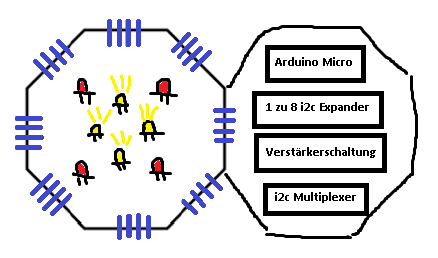
\includegraphics[scale=0.8]{../figures/OktokommanderOffen.png}
	\caption{\textcolor{red}{Erklärung!}}
	\label{fig:OktokommanderOffen}
\end{figure}

Um den Oktokommander mit den Detektormodulen erweitern zu können wurden USB-2A Schnittstellen verwendet. Durch diese Schnittstellen können bis zu 7 Detektormodule, jeweils eines pro Seite  eingekoppelt werden. Um eine größere Platte zu konstruieren können noch weitere Detektormodule an den bereits vorhandenen Detektormodule angeschlossen werden.
\textcolor{red}{Erklärung der Komponenten an Hand des Bildes}

\begin{figure}[h]
	\centering
	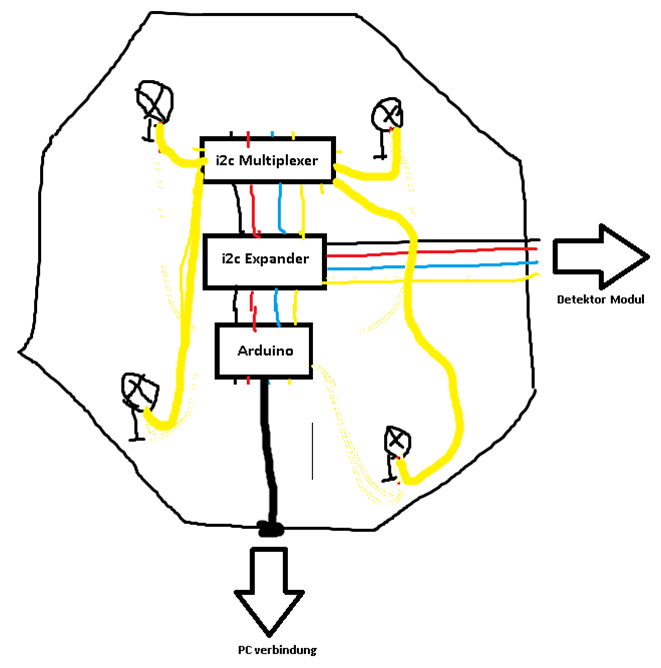
\includegraphics[scale=0.8]{../figures/PrinzipskizzeOktokommander.png} 
	\caption{\textcolor{red}{Erklärung!}}
	\label{fig:PrinzipskizzeOktokommander}
\end{figure}

% -------------------------------------------------------------------------------------- %

\section{Detektormodul}
\label{sec:Detektormodul}

Das Detektormodul besteht lediglich aus vier Photodioden und einem USB-2A Eingang. Dadurch kann das Detektormodul an den Oktokommander angeschlossen werden. Zur Ansteuerung der Photodioden wurde auch hier ein i2c Expander verwendet. 
\textcolor{red}{Erklärung der Komponenten der Bilder}

\begin{figure}[h]
	\centering
	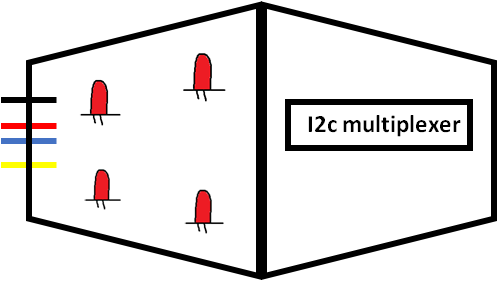
\includegraphics[scale=0.7]{../figures/DetektormodulOffen.png}
	\caption{\textcolor{red}{Erklärung!}}
	\label{fig:DetektormodulOffen}
\end{figure}

\begin{figure}[h]
	\centering
	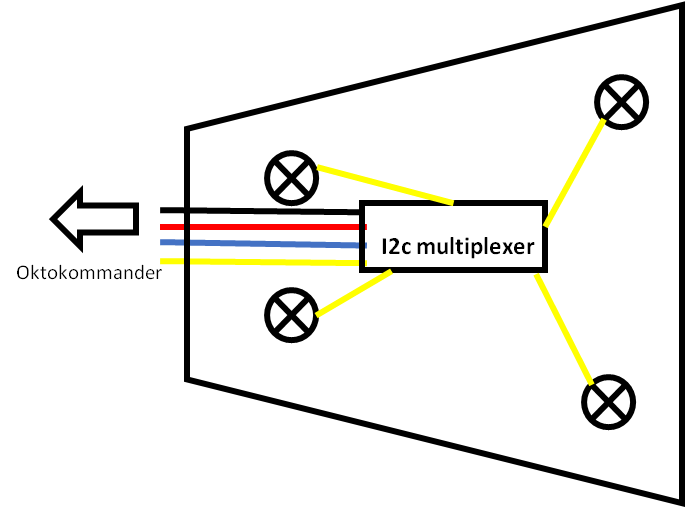
\includegraphics[scale=0.5]{../figures/PrinzipskizzeDetektormodul.png}
	\caption{\textcolor{red}{Erklärung!}}
	\label{fig:PrinzipskizzeDetektormodul}
\end{figure}

% -------------------------------------------------------------------------------------- %

\section{Software}
\label{sec:Software}

Die Software-Seite des Gestikulasers ist für die Zuordnung der Gesten zuständig. Die von den Detektormodulen gemessenen Reflektionsmuster werden an den Mikrocontroller im Oktokommander und von da aus an einen Computer weitergeleitet, wo sie verarbeitet werden. Bei der dazu eingesetzten Software wurde komplett auf open-source verfügbare Programme und Bibliotheken gesetzt. Der Code auf den Microcontrollern wurde mit Hilfe der \href{https://www.arduino.cc/en/Main/Software}{\texttt{Arduino IDE}} entwickelt. Die Verarbeitung am Computer erfolgt mit Hilfe von \texttt{Python} Skripten. Für den Machine Learning Teil wurde die \href{https://www.tensorflow.org/}{\texttt{TensorFlow}\texttrademark} Bibliothek verwendet. Die Software kann in zwei Teile unterteilt werden, die im Folgenden genauer erläutert werden.

\subsubsection*{Trainingsphase}
Der erste Teil der Software kommt während der Trainingsphase zum Einsatz. Hier werden die von den Photodioden gemessenen Daten aus dem Microcontroller im Oktokommander zunächst ausgelesen und gemeinsam mit einem Label, das der gerade aufgenommenen Geste entspricht, in eine Datei geschrieben. Die auf diese Weise gesammelten Daten werden dann im nächsten Schritt verwendet, um ein mathematisches Modell zu erstellen, das im Live-Betrieb angewendet wird, um die vom Nutzer gemachte Geste, einer der bekannten zuordnen zu können. Angenommen es stehen Daten von $N$ Photodioden zur Verfügung, dann können diese Daten in dem Vektor $x\in \mathbb{R}^N$ zusammengefasst werden. Für den Anfang soll ein Modell entwickelt werden, welches einem beliebigen gemessenen Datensatz $x$ eine der $m$ vordefinierten Gesten $G_1 , ... , G_m$ zuordnet. Dazu stellt der Nutzer vor Aufzeichnung der Daten in dem Python Skript ein, was für eine Geste $G_j$ er als nächstes aufnehmen will. Nachdem für jede Geste ausreichend Daten aufgenommen wurden, kann als nächstes das mathematische Modell erstellt werden, um die Sensordaten zu verarbeiten. Ziel ist es, ein gegebenes Datum $x_i$, das im Live-Betrieb gemessen wird, eindeutig einer Geste $G_j$ zuzuordnen. Damit Datum $x_i$ der Geste $G_j$ zugeordnet wird, muss die Bedingung 
\begin{align*}
	p(G_j | x_i) \geq p(G_k | x_i) \quad \forall k = 1,...,m \quad k \neq j
\end{align*}
erfüllt sein. Dabei ist $p(G_j | x_i)$ die bedingte Wahrscheinlichkeit für Geste $G_j$ gegeben die Photomessdaten $x_i$. Diese Bedingung lässt sich leicht überprüfen, allerdings ist die bedingte Wahrscheinlichkeit $p(G | x)$ unbekannt. Aus diesem Grund wird ein neuronales Netz mit Hilfe der zuvor aufgezeichneten Daten $(x,G) \in \mathbb{R}^N \times \mathbb{R}$ trainiert, das die unbekannte bedingte Wahrscheinlichkeit annähert. Der Aufbau und das Training des neuronalen Netzes erfolgen mit Hilfe vordefinierter Methoden von \texttt{TensorFlow}\texttrademark. Nach erfolgreich abgeschlossenem Training wird das neuronale Netz in eine Datei exportiert und kann nun im Live-Betrieb verwendet werden.

\subsubsection*{Live-Betrieb}
Im Live-Betrieb wird das zuvor trainierte Modell nun verwendet, um die nun unbekannten Reflektionsmuster, die von den Photodioden gemessen und über den Mikrocontroller an den PC weitergeleitet wurden, einer bekannten Geste zuzuordnen. Nachdem die gemessenen Daten einer Geste zugeordnet wurden, wird der mit dieser Geste verknüpfte Steuerungsbefehl bestimmt und an das angeschlossene Endgerät weitergeleitet. Dieser Ablauf ist in \reffig{fig:AblaufSteuerung} dargestellt.

\begin{figure}[h]
	\centering
	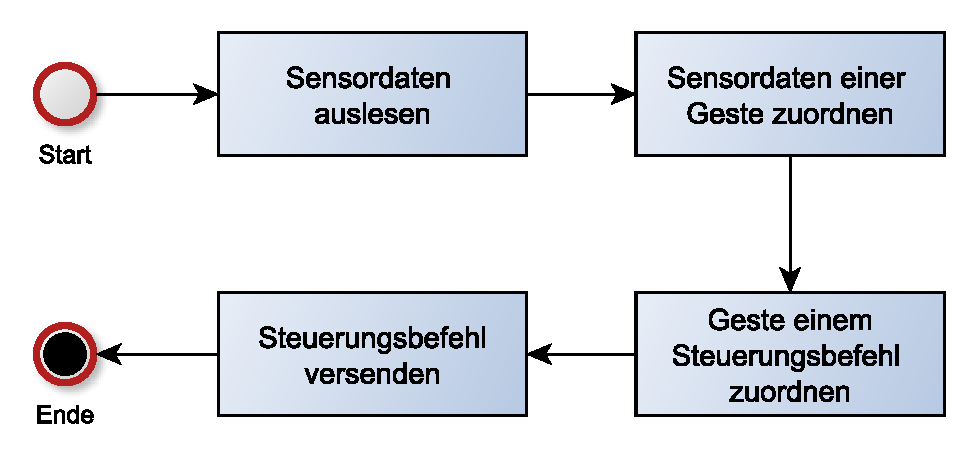
\includegraphics[scale=0.75]{../figures/AblaufSteuerung.pdf}
	\caption{Ablaufdiagramm der Software im Live-Betrieb: Die aus dem Microcontroller ausgelesenen Sensordaten werden zur Verarbeitung an das Python Skript übergeben, wo sie einer Geste und diese einem Steuerbefehl zugeordnet wird. Dieser Steuerungsbefehl wird schließlich an das anzusteuernde Endgerät weitergegeben.}
	\label{fig:AblaufSteuerung}
\end{figure}